%% abtex2-modelo-trabalho-academico.tex, v-1.9.7 laurocesar
%% Copyright 2012-2018 by abnTeX2 group at http://www.abntex.net.br/ 
%%
%% This work may be distributed and/or modified under the
%% conditions of the LaTeX Project Public License, either version 1.3
%% of this license or (at your option) any later version.
%% The latest version of this license is in
%%   http://www.latex-project.org/lppl.txt
%% and version 1.3 or later is part of all distributions of LaTeX
%% version 2005/12/01 or later.
%%
%% This work has the LPPL maintenance status `maintained'.
%% 
%% The Current Maintainer of this work is the abnTeX2 team, led
%% by Lauro César Araujo. Further information are available on 
%% http://www.abntex.net.br/
%%
%% This work consists of the files abntex2-modelo-trabalho-academico.tex,
%% abntex2-modelo-include-comandos and abntex2-modelo-references.bib
%%

% ------------------------------------------------------------------------
% ------------------------------------------------------------------------
% abnTeX2: Modelo de Trabalho Academico (tese de doutorado, dissertacao de
% mestrado e trabalhos monograficos em geral) em conformidade com 
% ABNT NBR 14724:2011: Informacao e documentacao - Trabalhos academicos -
% Apresentacao
% ------------------------------------------------------------------------
% ------------------------------------------------------------------------

\documentclass[
	% -- opções da classe memoir --
	12pt,				% tamanho da fonte
	openright,			% capítulos começam em pág ímpar (insere página vazia caso preciso)
	oneside,			    % para impressão em recto e verso usar two side (Oposto a oneside)
	a4paper,				% tamanho do papel. 
	% -- opções da classe abntex2 --
	%chapter=TITLE,		% títulos de capítulos convertidos em letras maiúsculas
	%section=TITLE,		% títulos de seções convertidos em letras maiúsculas
	%subsection=TITLE,	% títulos de subseções convertidos em letras maiúsculas
	%subsubsection=TITLE,% títulos de subsubseções convertidos em letras maiúsculas
	% -- opções do pacote babel --
	english,			% idioma adicional para hifenização
	french,			% idioma adicional para hifenização
	spanish,			% idioma adicional para hifenização
	brazil			% o último idioma é o principal do documento
	]{abntex2}

% ---
% Pacotes básicos 
% ---
\usepackage{lmodern}			% Usa a fonte Latin Modern			
\usepackage[T1]{fontenc}		% Selecao de codigos de fonte.
\usepackage[utf8]{inputenc}	% Codificacao do documento (conversão automática dos acentos)
\usepackage{indentfirst}		% Indenta o primeiro parágrafo de cada seção.
\usepackage{color}			% Controle das cores
\usepackage{graphicx}		% Inclusão de gráficos
\usepackage{microtype} 		% para melhorias de justificação
% ---
		
% ---
% Pacotes adicionais, usados apenas no âmbito do Modelo Canônico do abnteX2
% ---
%\usepackage{lipsum}				% para geração de dummy text
% ---

% ---
% Pacotes de citações
% ---
\usepackage[brazilian,hyperpageref]{backref}	 % Paginas com as citações na bibl
\usepackage[alf]{abntex2cite}	% Citações padrão ABNT

% --- 
% CONFIGURAÇÕES DE PACOTES
% --- 

% ---
% Configurações do pacote backref
% Usado sem a opção hyperpageref de backref
% \renewcommand{\backrefpagesname}{Citado na(s) página(s):~}
% Texto padrão antes do número das páginas
%\renewcommand{\backref}{}
% Define os textos da citação
%\renewcommand*{\backrefalt}[4]{
%	\ifcase #1 %
%		Nenhuma citação no texto.%
%	\or
%		Citado na página #2.%
%	\else
%		Citado #1 vezes nas páginas #2.%
%	\fi}%
% ---

% ---
% Informações de dados para CAPA e FOLHA DE ROSTO
% ---
\titulo{Ion-Note}
\author{Pedro Figueiredo Dias - 41990455, Nathan Silva Macena - 41990404, Lucas Alexandre Arruda Lira - 41547241}
\local{Brasil}
\data{2022}
\orientador{Lauro César Araujo}
\coorientador{Equipe \abnTeX}
\instituicao{%
  Universidade Presbiteriana Mackenzie -- UPM
  \par
  Faculdade de Computação e Informática
  \par
  Programa de Graduação}
\tipotrabalho{Tese (Doutorado)}
% O preambulo deve conter o tipo do trabalho, o objetivo, 
% o nome da instituição e a área de concentração 
\preambulo{Modelo canônico de trabalho monográfico acadêmico em conformidade com
as normas ABNT apresentado à comunidade de usuários \LaTeX.}
% ---


% ---
% Configurações de aparência do PDF final

% alterando o aspecto da cor azul
\definecolor{blue}{RGB}{41,5,195}

% informações do PDF
\makeatletter
\hypersetup{
     	%pagebackref=true,
		pdftitle={\@title}, 
		pdfauthor={\@author},
    		pdfsubject={\imprimirpreambulo},
	    pdfcreator={LaTeX with abnTeX2},
		pdfkeywords={abnt}{latex}{abntex}{abntex2}{trabalho acadêmico}, 
		colorlinks=true,       	% false: boxed links; true: colored links
    		linkcolor=blue,          % color of internal links
    		citecolor=blue,        	% color of links to bibliography
    		filecolor=magenta,      	% color of file links
		urlcolor=blue,
		bookmarksdepth=4
}
\makeatother
% --- 

% ---
% Posiciona figuras e tabelas no topo da página quando adicionadas sozinhas
% em um página em branco. Ver https://github.com/abntex/abntex2/issues/170
\makeatletter
\setlength{\@fptop}{5pt} % Set distance from top of page to first float
\makeatother
% ---

% ---
% Possibilita criação de Quadros e Lista de quadros.
% Ver https://github.com/abntex/abntex2/issues/176
%
\newcommand{\quadroname}{Quadro}
\newcommand{\listofquadrosname}{Lista de quadros}

\newfloat[chapter]{quadro}{loq}{\quadroname}
\newlistof{listofquadros}{loq}{\listofquadrosname}
\newlistentry{quadro}{loq}{0}

% configurações para atender às regras da ABNT
\setfloatadjustment{quadro}{\centering}
\counterwithout{quadro}{chapter}
\renewcommand{\cftquadroname}{\quadroname\space} 
\renewcommand*{\cftquadroaftersnum}{\hfill--\hfill}

\setfloatlocations{quadro}{hbtp} % Ver https://github.com/abntex/abntex2/issues/176
% ---

% --- 
% Espaçamentos entre linhas e parágrafos 
% --- 

% O tamanho do parágrafo é dado por:
\setlength{\parindent}{1.3cm}

% Controle do espaçamento entre um parágrafo e outro:
\setlength{\parskip}{0.2cm}  % tente também \onelineskip

% ---
% compila o indice
% ---
\makeindex
% ---

% ----
% Início do documento
% ----
\begin{document}

% Seleciona o idioma do documento (conforme pacotes do babel)
%\selectlanguage{english}
\selectlanguage{brazil}

% Retira espaço extra obsoleto entre as frases.
\frenchspacing 

% ----------------------------------------------------------
% ELEMENTOS PRÉ-TEXTUAIS
% ----------------------------------------------------------
% \pretextual

% ---
% Capa
% ---
\imprimircapa
% ---

% ---
% inserir o sumario
% ---
\pdfbookmark[0]{\contentsname}{toc}
\tableofcontents*
\cleardoublepage
% ---



% ----------------------------------------------------------
% ELEMENTOS TEXTUAIS
% ----------------------------------------------------------
\textual

% ----------------------------------------------------------
\chapter{Introdução}
Documentação do projeto elaborado e desenvolvido na disciplina de Laboratório de Engenharia de Software.
\chapter{Descrição do projeto}
\section{O problema ou oportunidade percebida}
Uma forma gratuita de organizar tarefas e anotações focada no público universitário.
\section{A razão ou justificativa para esta demanda}
Em meio a atualidade de plataformas e serviços que prometem auxiliar na organização de anotações e tarefas, sentimos a falta de uma solução gratuita e eficaz voltada a universitários.
\section{A descrição sucinta do produto de software que será produzido}
Um gerenciador WEB de notas e tarefas, capaz de importar tarefas da plataforma Moodle.
\section{Identifique os clientes, usuários e demais envolvidos/impactados com o produto}
Universitários e profissionais da área de tecnologia.
\section{Descreva, em linhas gerais, quais as principais etapas necessárias para construir este produto}
1 - Entender o funcionamento dos arquivos referentes a importação dos calendários;

2 - Iniciar os testes com os arquivos lidos pelo calendário;

3 - Construir um protótipo com a interface da aplicação;

4 - Construir um protótipo funcional da aplicação;

5 - Iniciar os testes de funcionalidade da aplicação;

6 - Finalizar a interface e a usabilidade da aplicação;

7 - Realizar toque finais na aplicação.
\section{Identifique os principais critérios de qualidade para o produto}
Nosso critério de qualidade é referente a fácil usabilidade da aplicação pelo cliente.
\chapter{Levantamentos de requisitos}
\section{Requisitos funcionais}
\begin{enumerate}
    \item Possibilidade de gerenciar de notas;
    \item Possibilidade de gerenciar de tarefas;
    \item Possibilidade de gerenciar de eventos;
    \item Deve ser capaz de autenticar um usuário;
    \item Deve ser capaz de limitar o acesso de um usuário a somente os artefatos vinculados a ele.
    \item Deve ser capaz de colher a lista de tarefas do Moodle;
    \item Deve ser capaz de atualizar esta lista automaticamente;
    \item Acesso a históricos de dados e informações pelos usuários;
    \item Opção de compartilhamento e trocas de informações entre os usuários;
\end{enumerate}

\section{Requisitos não funcionais}
\begin{enumerate}
    \item Deve possuir um interface simples;
    \item Deve ser customizável.
\end{enumerate}

\chapter{Modelagem de sistema}
\section{Casos de uso}
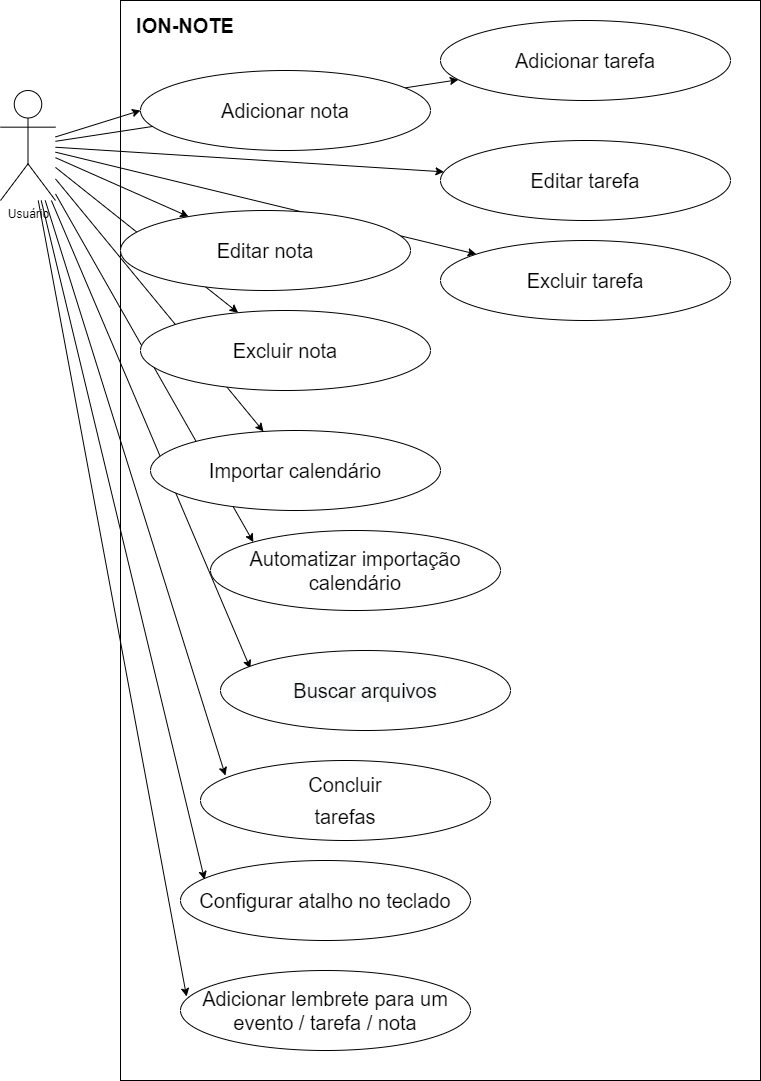
\includegraphics[scale=0.4]{Imagens/Casos-de-uso.jpeg}

\section{Especificação de casos de uso}
\subsection{Adicionar anotação}
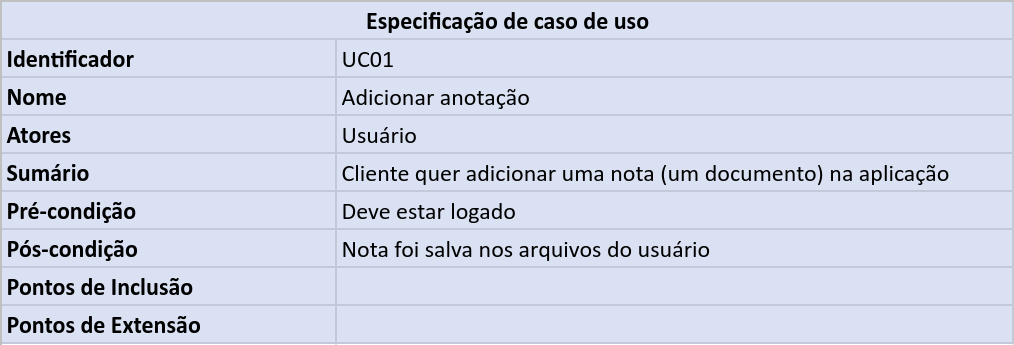
\includegraphics[scale=0.4]{Imagens/UC1-DESC.png}

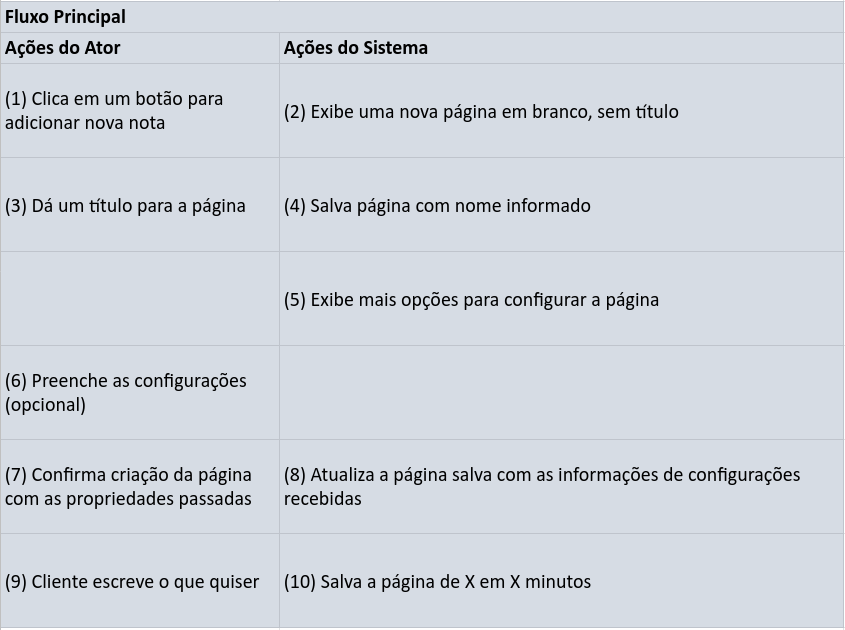
\includegraphics[scale=0.4]{Imagens/UC1-FP.png}

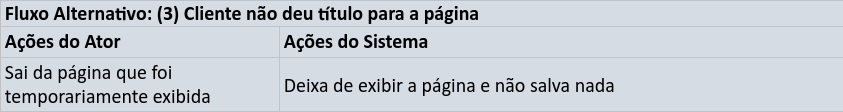
\includegraphics[scale=0.4]{Imagens/UC1-FA1.png}

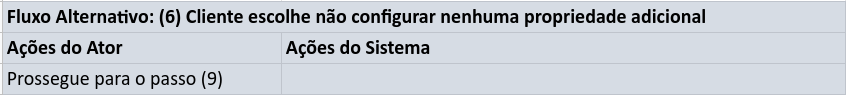
\includegraphics[scale=0.4]{Imagens/UC1-FA2.png}

\subsection{Importar calendário}
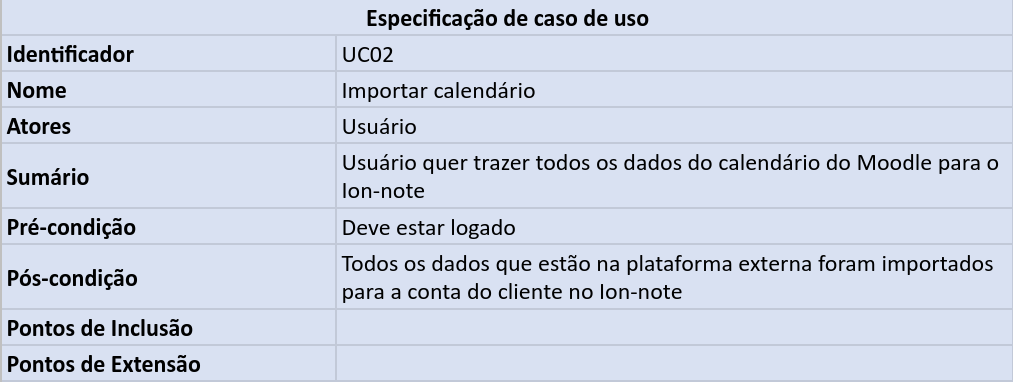
\includegraphics[scale=0.4]{Imagens/UC2-DESC.png}

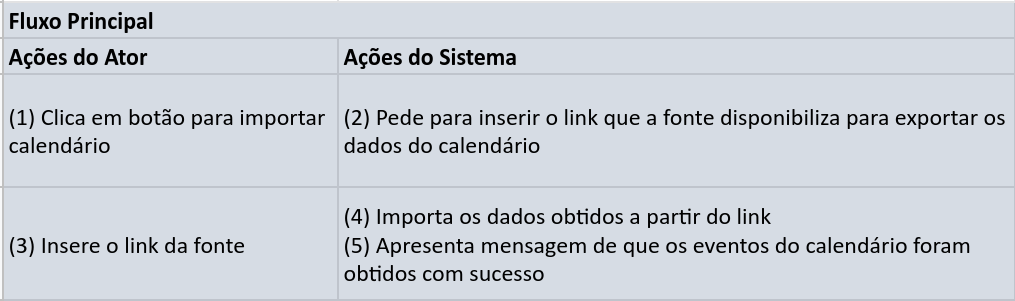
\includegraphics[scale=0.4]{Imagens/UC2-FP.png}

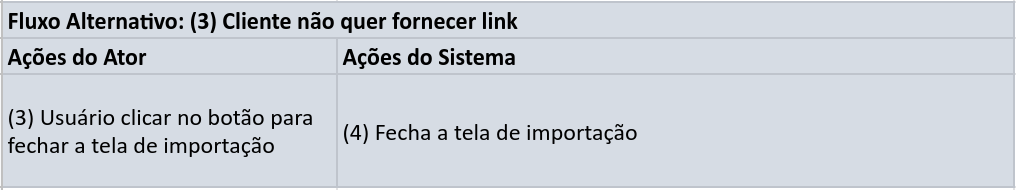
\includegraphics[scale=0.4]{Imagens/UC2-FA1.png}

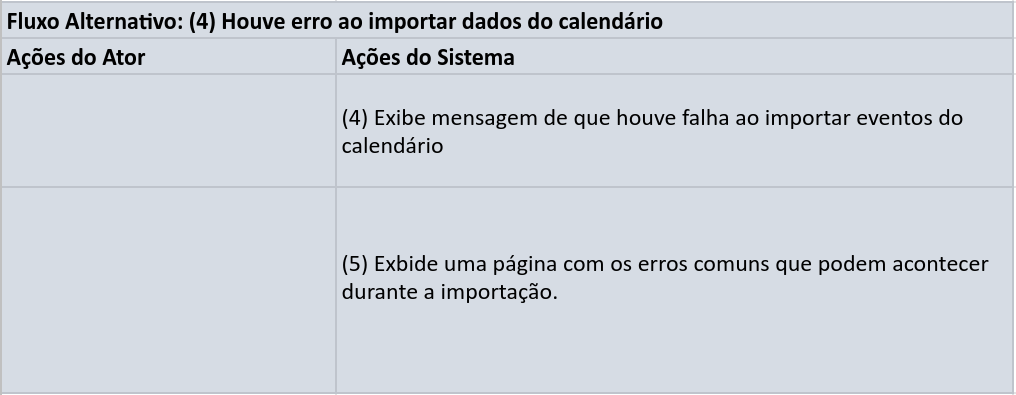
\includegraphics[scale=0.4]{Imagens/UC2-FA2.png}




\section{Diagramas de sequência}
\subsection{Adicionar anotação}
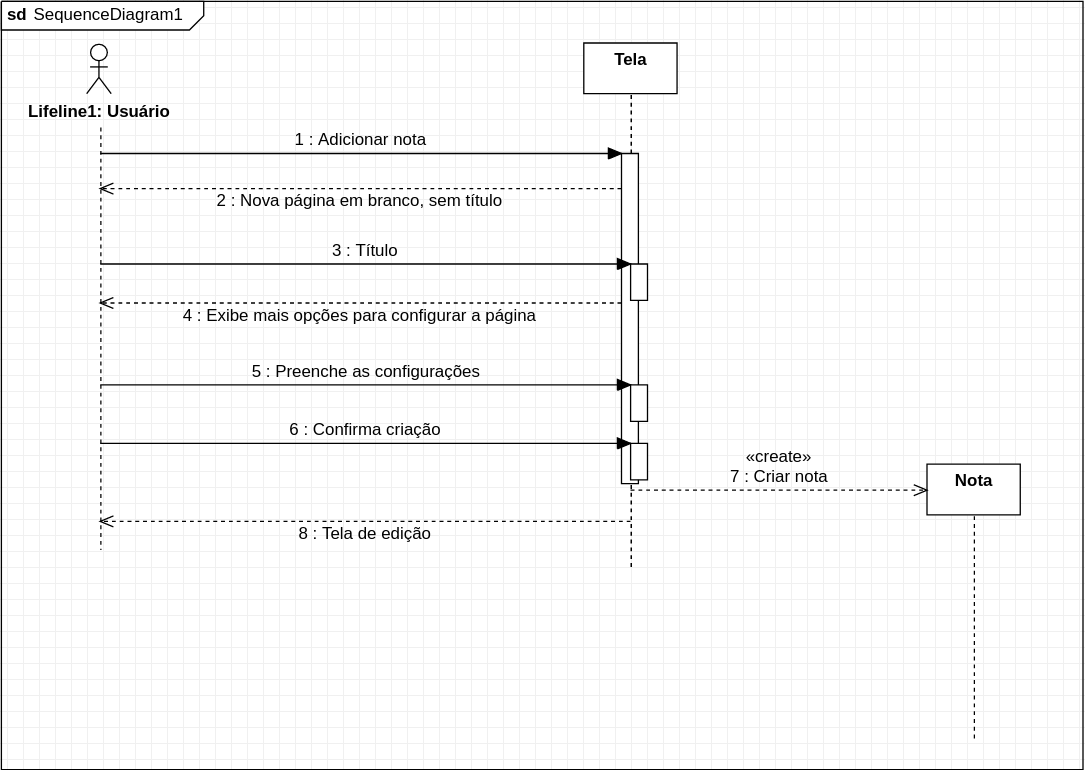
\includegraphics[scale=0.4]{Imagens/UC1-SEQ.png}

\subsection{Importar calendário}
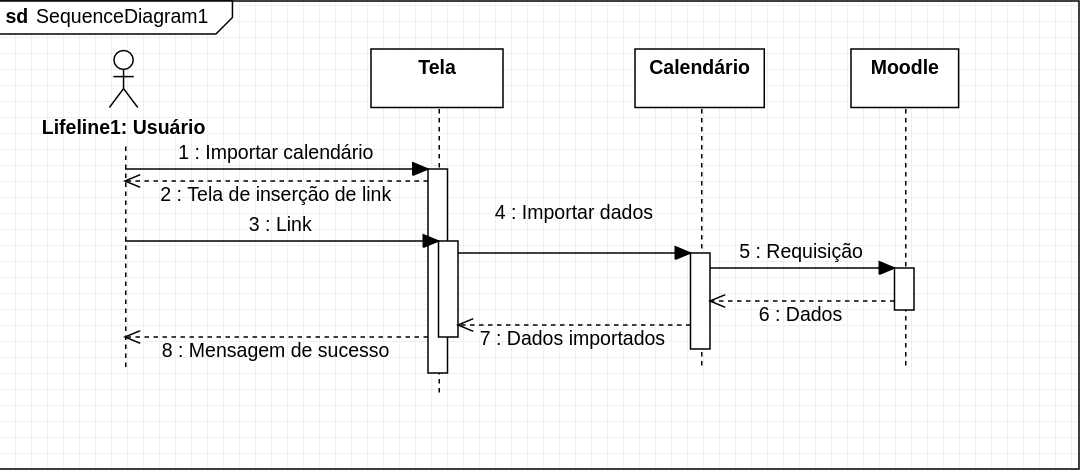
\includegraphics[scale=0.4]{Imagens/UC2-SEQ.png}

\section{Diagrama de classes}
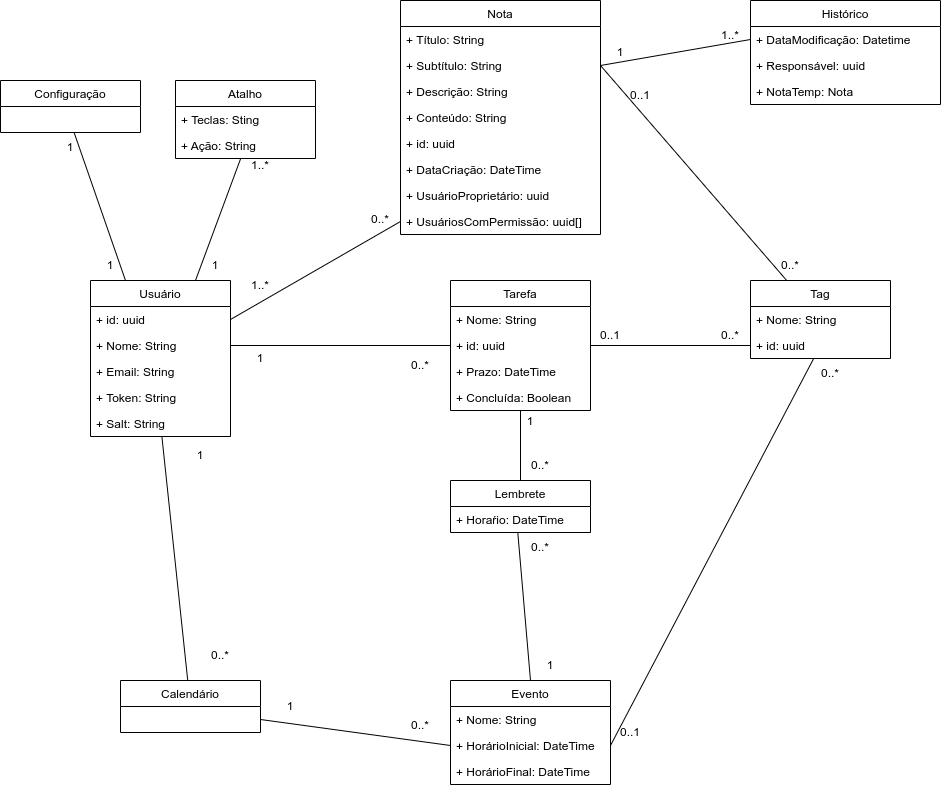
\includegraphics[scale=0.4]{Imagens/diagramaClasse.drawio.png}

\chapter{Wireframe}
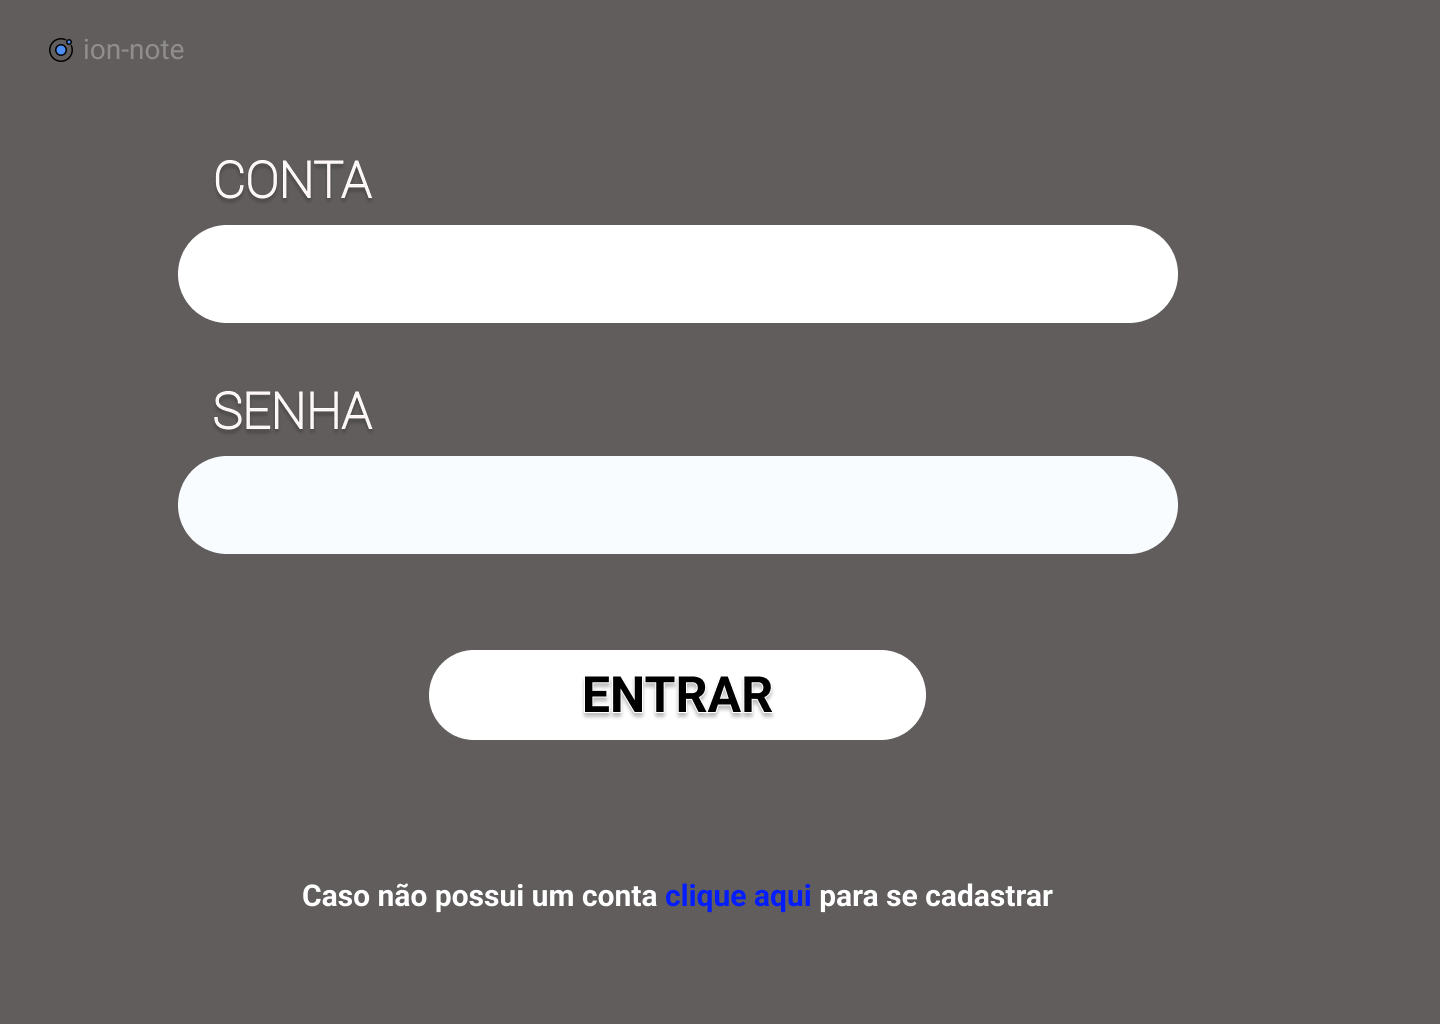
\includegraphics[scale=0.3]{Imagens/Login.png}

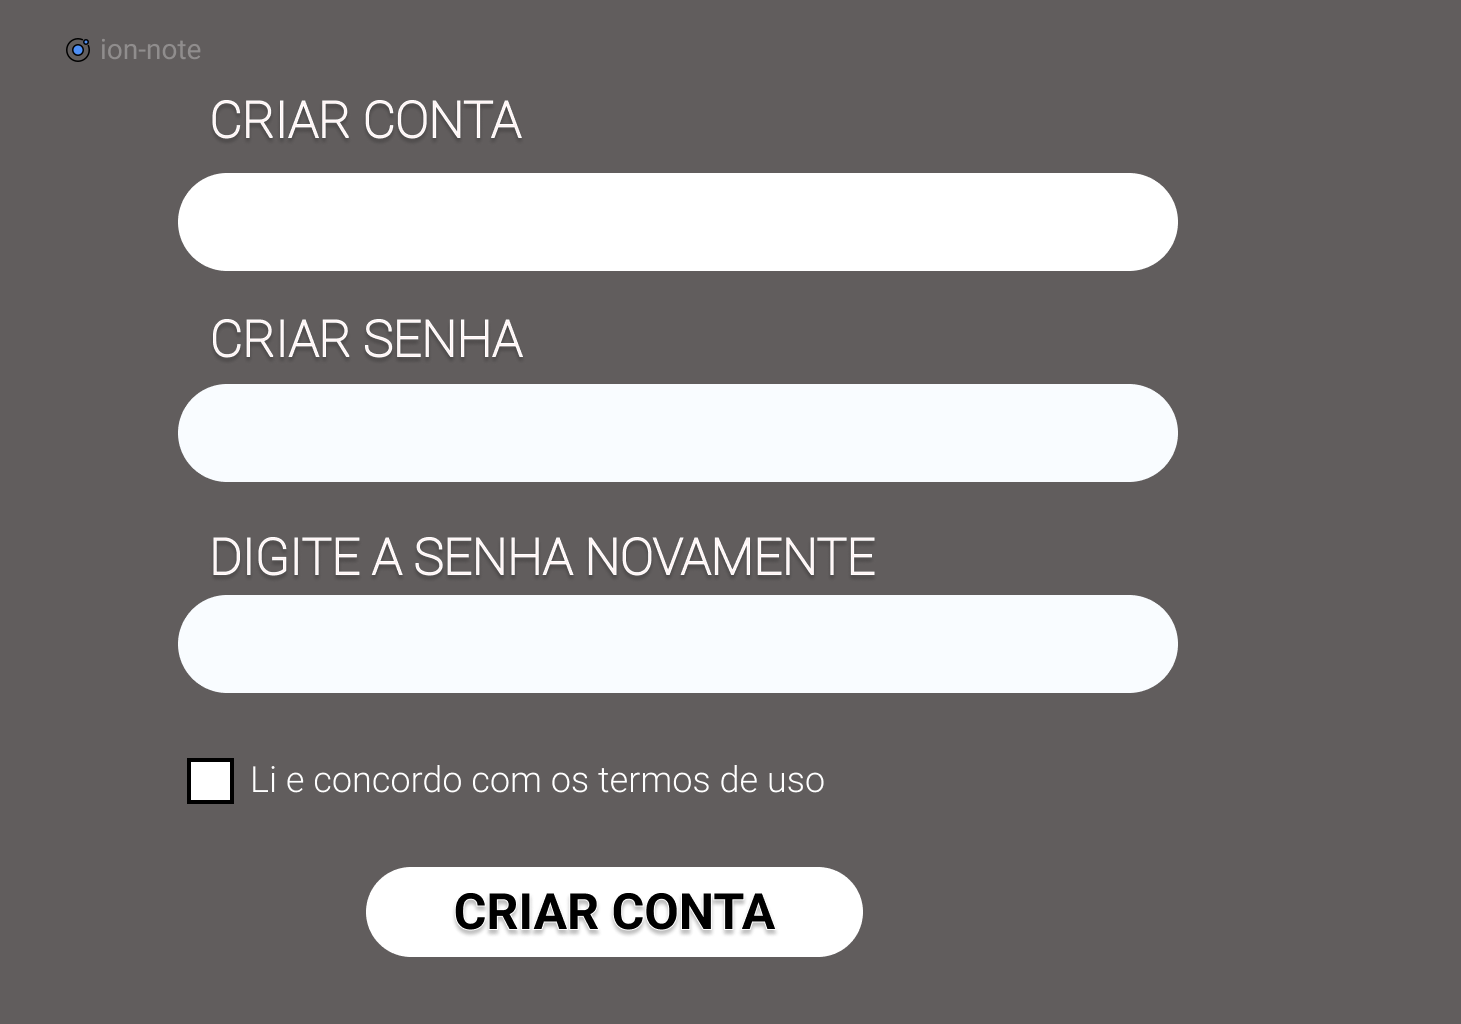
\includegraphics[scale=0.3]{Imagens/Criar conta.png}

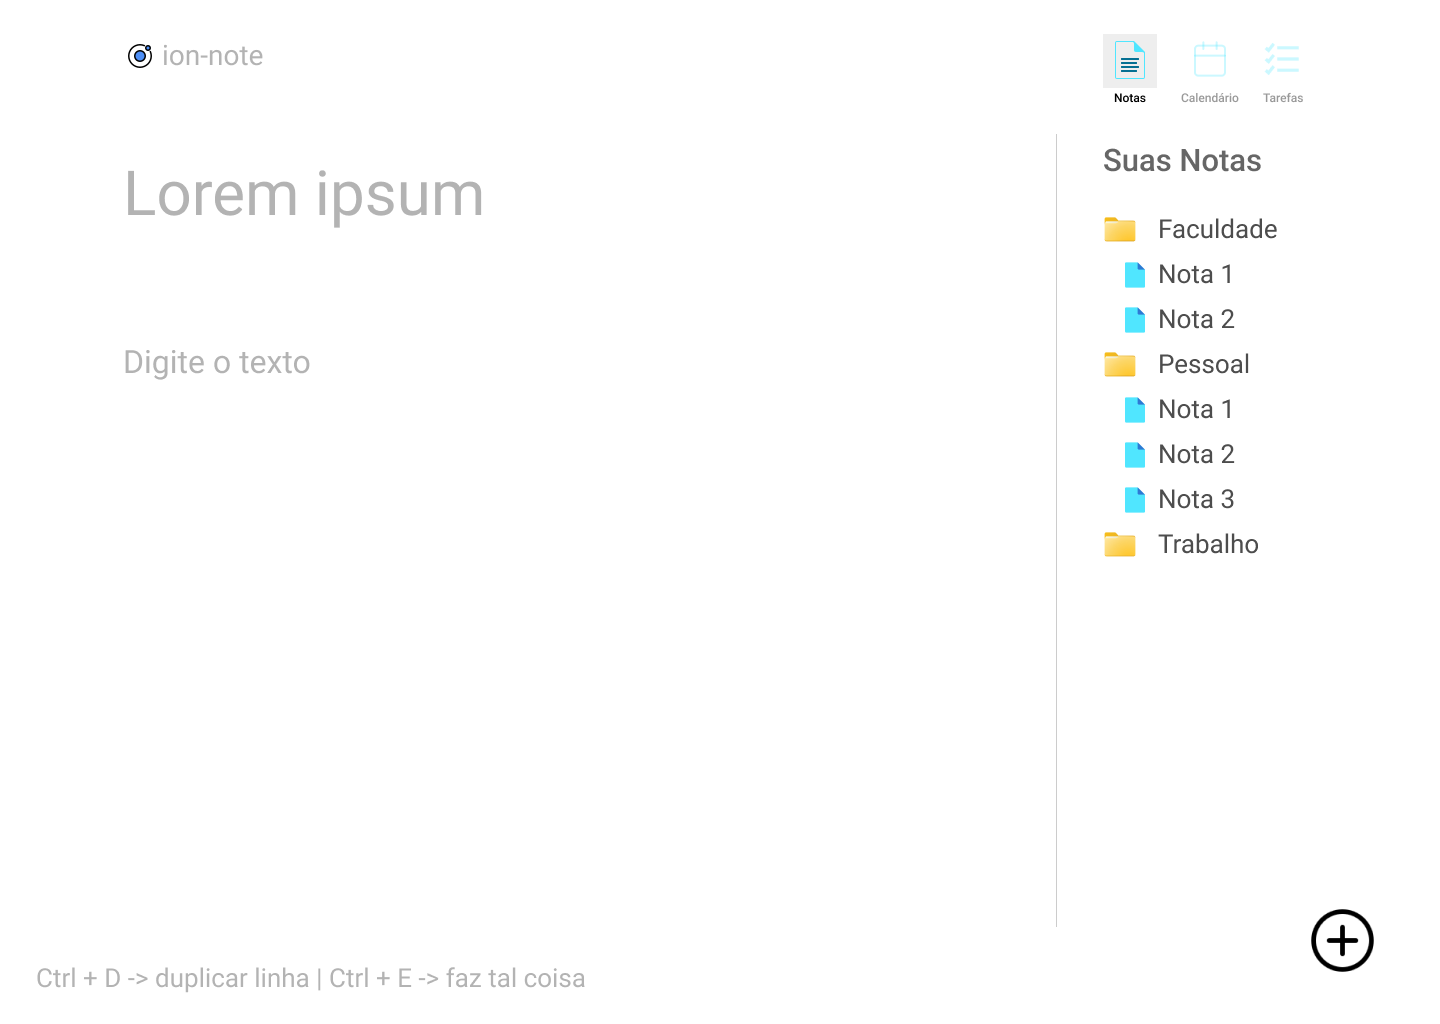
\includegraphics[scale=0.3]{Imagens/Adicionar nota.png}

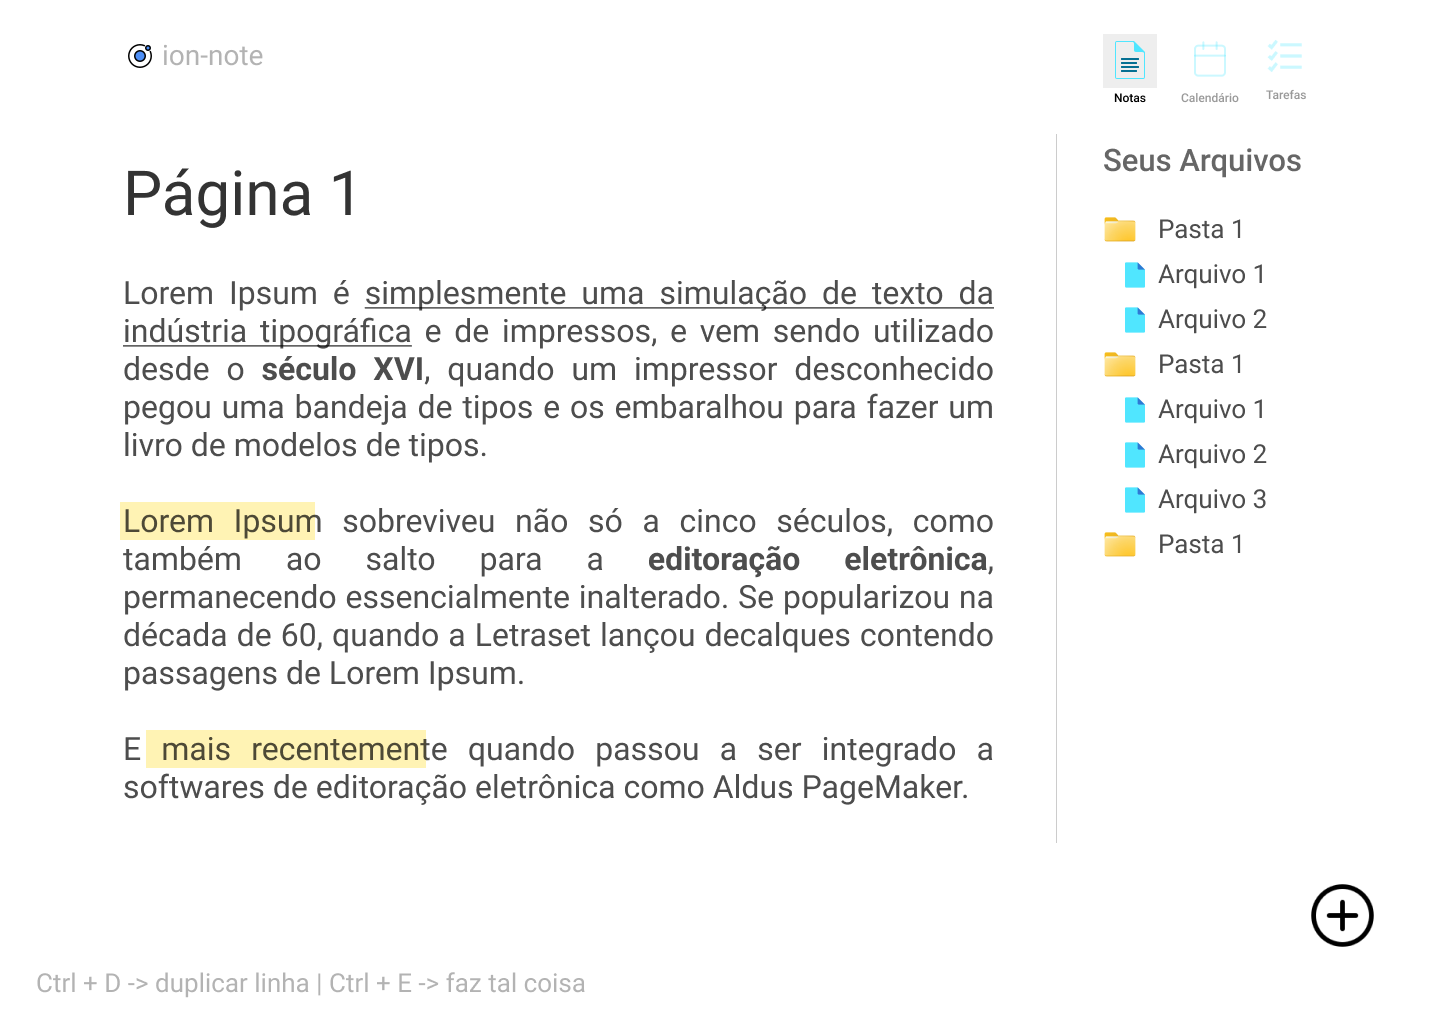
\includegraphics[scale=0.3]{Imagens/Nota preenchida.png}

\includegraphics[scale=0.3]{Imagens/Calendário.png}

\includegraphics[scale=0.3]{Imagens/Calendário - adicionar lembrete}

\includegraphics[scale=0.3]{Imagens/Calendário - importar.png}

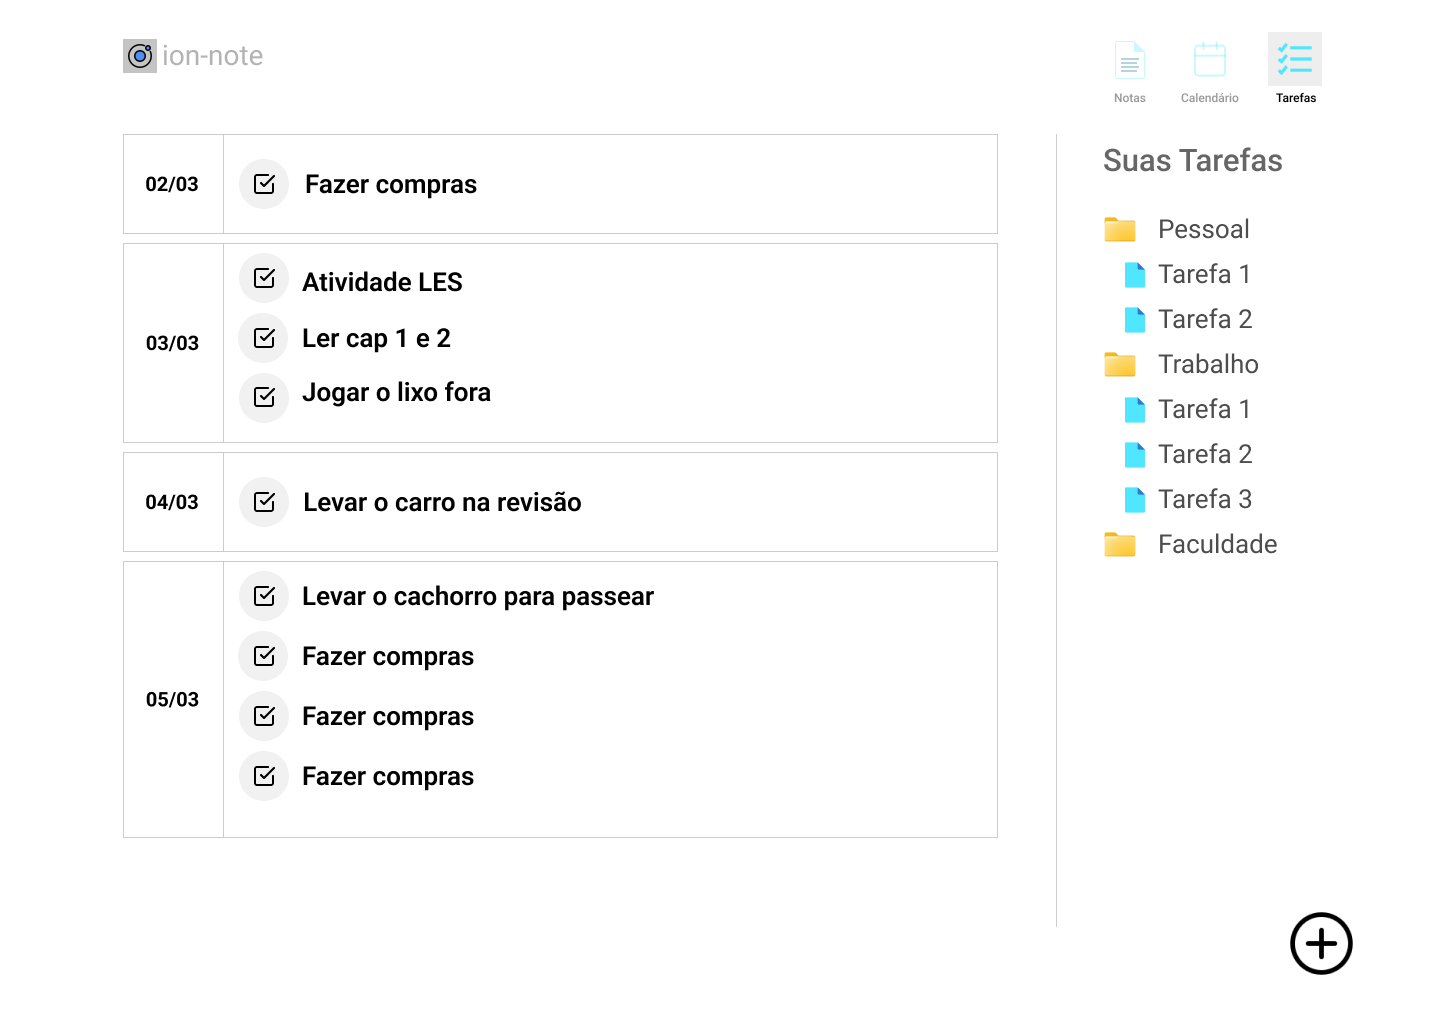
\includegraphics[scale=0.3]{Imagens/Tarefa.png}

\chapter{Arquitetura}
\section{Descrição}
Após analisar a proposta da aplicação decidimos utilizar uma arquitetura em camadas e as seguintes tecnologias:
\subsection{FrontEnd}
\begin{itemize}
    \item \textbf{React.}
\end{itemize}

\subsection{BackEnd}
\begin{itemize}
    \item \textbf{Java;}
    \item \textbf{SpringBoot;}
    \item \textbf{PostgreSQL;}
    \item \textbf{MongoDB.}
\end{itemize}

\subsection{Arquitetura}
A arquitetura escolhida é composta pelas seguintes camadas e funções:
\begin{itemize}
    \item \textbf{Controllers}: São os componentes mais externos, mas especificamente os endpoints da aplicação;
    \item \textbf{Services}: São os componentes responsáveis por implmentar as regras de negócios utilizando classes Entities e Repositories;
    \item \textbf{Entities}: São as classes que modelam as entidades necessárias para a aplicação;
    \item \textbf{Repositories}: São interfaces CRUD para com os sistemas de persistência escolhidos.
\end{itemize}

\section{Diagrama}
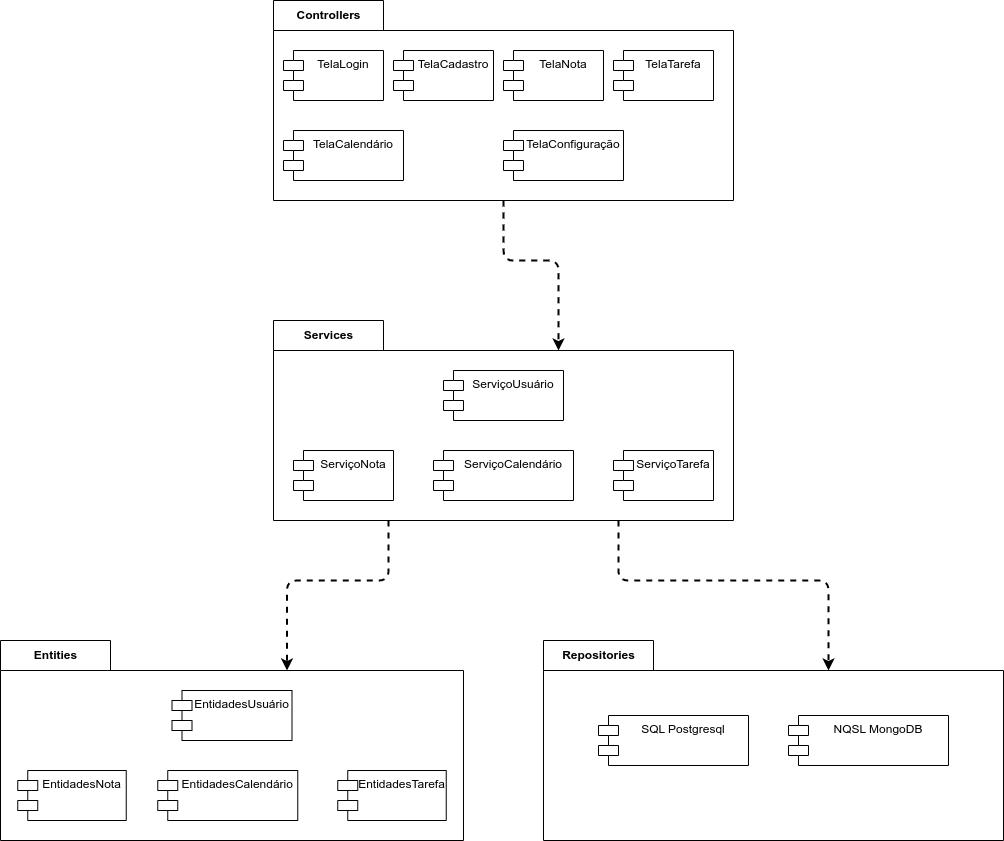
\includegraphics[scale=0.4]{Imagens/arquitetura.png}


\end{document}
